% Generated by scripts/campaign/paper_figures.py --docs; do not edit.

\section*{Figures}
{\footnotesize\begin{itemize}\setlength{\itemsep}{0pt}
\item[] \textit{System Design}
\item Fig.~\ref{fig:arch}: \texttt{arch}, double
\item[] \textit{System Design: Placement}
\item Fig.~\ref{fig:placement}: \texttt{placement}, single
\item Fig.~\ref{fig:lease}: \texttt{lease}, single
\item[] \textit{System Design: Environment Reproduction}
\item Fig.~\ref{fig:closure}: \texttt{closure}, single
\item[] \textit{System Design: Joining Across Networks}
\item Fig.~\ref{fig:nat}: \texttt{nat}, single
\item Fig.~\ref{fig:trust}: \texttt{trust}, single
\item[] \textit{System Design: Transparent Interception}
\item Fig.~\ref{fig:shim}: \texttt{shim}, double
\item Fig.~\ref{fig:shuffle}: \texttt{shuffle}, single
\item Fig.~\ref{fig:ddp}: \texttt{ddp}, single
\item[] \textit{System Design: The Cost Model}
\item Fig.~\ref{fig:cost}: \texttt{cost}, single
\item[] \textit{System Design: Implementation}
\item Fig.~\ref{fig:sandbox}: \texttt{sandbox}, single
\item[] \textit{Evaluation: Setup}
\item Fig.~\ref{fig:lab}: \texttt{lab}, double
\item Fig.~\ref{fig:eval-e14-staircase}: \texttt{eval-e14-staircase}, single
\item Fig.~\ref{fig:eval-e17-ready}: \texttt{eval-e17-ready}, single
\item[] \textit{Evaluation: Microbenchmarks (Q1, Q2)}
\item Fig.~\ref{fig:eval-e7-overhead-cdf}: \texttt{eval-e7-overhead-cdf}, single
\item Fig.~\ref{fig:eval-time-breakdown}: \texttt{eval-time-breakdown}, single
\item Fig.~\ref{fig:eval-e17-footprint}: \texttt{eval-e17-footprint}, single
\item Fig.~\ref{fig:eval-e19-ship}: \texttt{eval-e19-ship}, single
\item[] \textit{Evaluation: End-to-end runs (Q3)}
\item Fig.~\ref{fig:eval-frontier}: \texttt{eval-frontier}, single
\item Fig.~\ref{fig:eval-strong-scaling}: \texttt{eval-strong-scaling}, double
\item Fig.~\ref{fig:eval-weak-scaling}: \texttt{eval-weak-scaling}, single
\item Fig.~\ref{fig:eval-wall-time}: \texttt{eval-wall-time}, double
\item Fig.~\ref{fig:eval-efficiency-heatmap}: \texttt{eval-efficiency-heatmap}, single
\item Fig.~\ref{fig:eval-e4-heterogeneous}: \texttt{eval-e4-heterogeneous}, single
\item Fig.~\ref{fig:eval-e6-kill}: \texttt{eval-e6-kill}, single
\item Fig.~\ref{fig:eval-cpu-heatmap}: \texttt{eval-cpu-heatmap}, double
\item Fig.~\ref{fig:eval-swimlanes}: \texttt{eval-swimlanes}, double
\item Fig.~\ref{fig:eval-net-bytes}: \texttt{eval-net-bytes}, single
\item Fig.~\ref{fig:eval-offload-share}: \texttt{eval-offload-share}, single
\item Fig.~\ref{fig:eval-e12-join}: \texttt{eval-e12-join}, double
\item Fig.~\ref{fig:eval-e13-churn}: \texttt{eval-e13-churn}, double
\item Fig.~\ref{fig:eval-e15-network}: \texttt{eval-e15-network}, single
\item Fig.~\ref{fig:eval-e16-energy}: \texttt{eval-e16-energy}, double
\item Fig.~\ref{fig:eval-e18-straggler}: \texttt{eval-e18-straggler}, double
\item Fig.~\ref{fig:eval-e20-unmodified}: \texttt{eval-e20-unmodified}, single
\item[] \textit{Evaluation: Training (Q4)}
\item Fig.~\ref{fig:eval-e8-training}: \texttt{eval-e8-training}, double
\end{itemize}}

\begin{figure*}[!t]
\centering
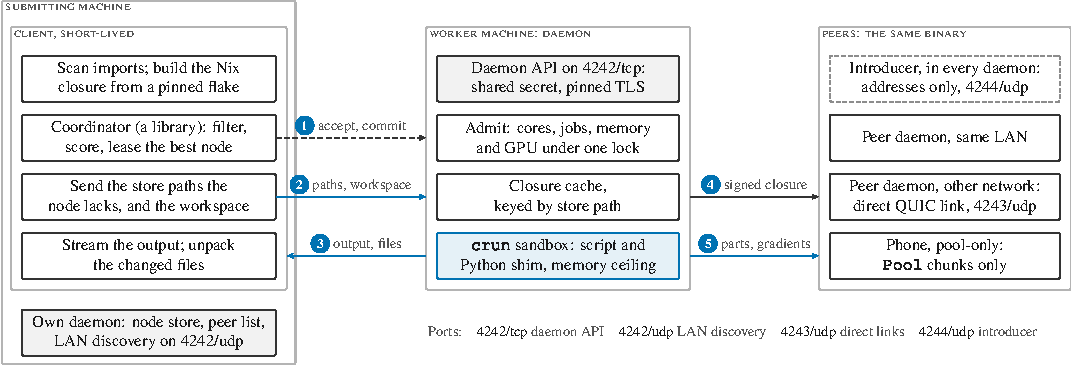
\includegraphics{../diagrams/tikz/pdf/arch.pdf}
\par\vspace{2pt}{\color{black!55}\scriptsize\texttt{arch}: double column, 7.14$\times$2.43\,in, System Design}
\caption{System design. Both roles are one binary. The client builds the closure, takes a lease (1) and sends only the store paths the worker lacks (2); output and changed files stream back (3). The worker pushes the signed closure to peers (4) and the shim spreads parts and gradients over them (5). Introducers carry addresses, never job data.}
\label{fig:arch}
\end{figure*}

\begin{figure}[!htb]
\centering
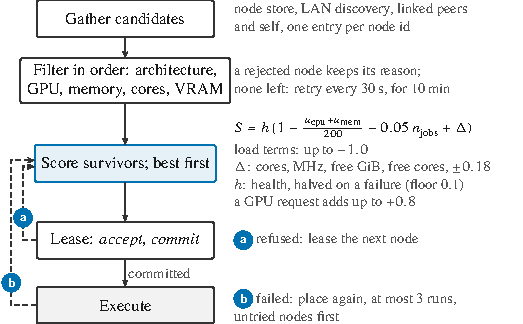
\includegraphics{../diagrams/tikz/pdf/placement.pdf}
\par\vspace{2pt}{\color{black!55}\scriptsize\texttt{placement}: single column, 3.49$\times$2.16\,in, System Design: Placement}
\caption{Placement in the submitting client. Hard filters run in order; survivors are ranked by the score S of Equation 1. A refused lease moves to the next node (a); a failed run is placed again, at most three times (b).}
\label{fig:placement}
\end{figure}

\begin{figure}[!htb]
\centering
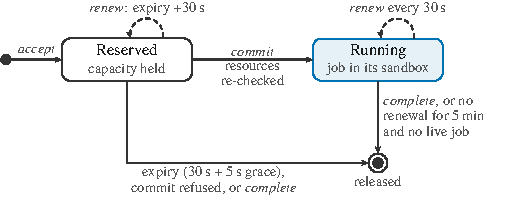
\includegraphics{../diagrams/tikz/pdf/lease.pdf}
\par\vspace{2pt}{\color{black!55}\scriptsize\texttt{lease}: single column, 3.49$\times$1.31\,in, System Design: Placement}
\caption{Lease states on the worker. A reservation expires 30 s after its last renewal plus a 5 s grace; a running lease is kept while its job lives and reaped only after 5 minutes without renewal.}
\label{fig:lease}
\end{figure}

\begin{figure}[!htb]
\centering
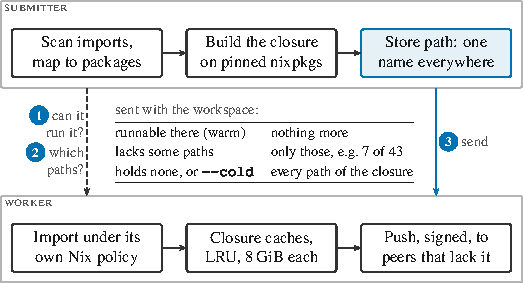
\includegraphics{../diagrams/tikz/pdf/closure.pdf}
\par\vspace{2pt}{\color{black!55}\scriptsize\texttt{closure}: single column, 3.49$\times$1.88\,in, System Design: Environment Reproduction}
\caption{Environment transfer. The client asks whether the worker can run the closure (1) and which store paths it lacks (2), and sends only those (3). Adding one package sent 7 of 43 paths, 28.6 MB of 206.0 MB.}
\label{fig:closure}
\end{figure}

\begin{figure}[!htb]
\centering
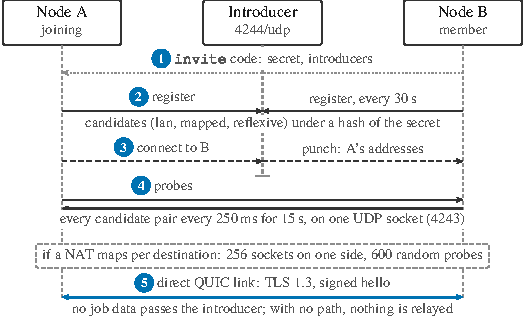
\includegraphics{../diagrams/tikz/pdf/nat.pdf}
\par\vspace{2pt}{\color{black!55}\scriptsize\texttt{nat}: single column, 3.49$\times$2.12\,in, System Design: Joining Across Networks}
\caption{Joining across networks. Both nodes register their candidates with an introducer (2), which forwards one punch request (3); both sides then probe every candidate pair (4) until a direct QUIC link forms (5). No job data passes through the introducer.}
\label{fig:nat}
\end{figure}

\begin{figure}[!htb]
\centering
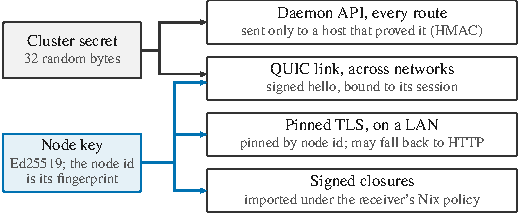
\includegraphics{../diagrams/tikz/pdf/trust.pdf}
\par\vspace{2pt}{\color{black!55}\scriptsize\texttt{trust}: single column, 3.49$\times$1.42\,in, System Design: Joining Across Networks}
\caption{Trust. The cluster secret guards every daemon route and the QUIC hello; the node key makes the TLS certificate, signs the hello and signs closures.}
\label{fig:trust}
\end{figure}

\begin{figure*}[!t]
\centering
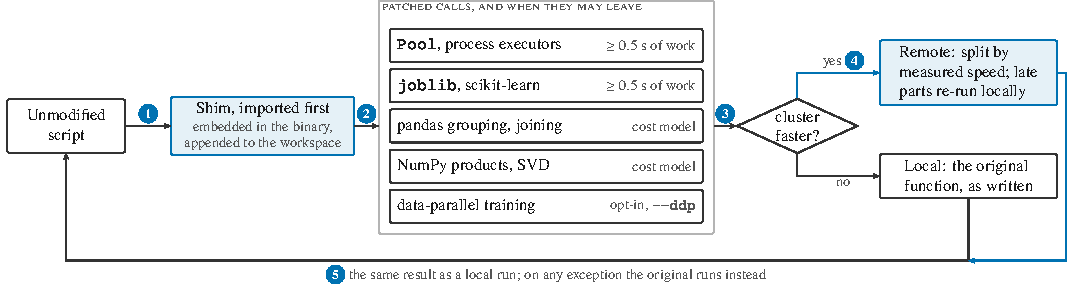
\includegraphics{../diagrams/tikz/pdf/shim.pdf}
\par\vspace{2pt}{\color{black!55}\scriptsize\texttt{shim}: double column, 7.14$\times$1.92\,in, System Design: Transparent Interception}
\caption{Transparent interception. The shim is imported before the script's first line (1) and patches the listed calls (2). Each call is gated (3); offloaded work is split by measured speed while local cores re-run late parts (4), and the script receives the result a local run would give (5).}
\label{fig:shim}
\end{figure*}

\begin{figure}[!htb]
\centering
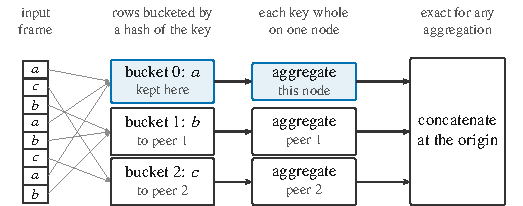
\includegraphics{../diagrams/tikz/pdf/shuffle.pdf}
\par\vspace{2pt}{\color{black!55}\scriptsize\texttt{shuffle}: single column, 3.49$\times$1.37\,in, System Design: Transparent Interception}
\caption{Hash shuffle for pandas grouping and joining. Rows are bucketed by a hash of their key, so each key is complete on one node and any aggregation is exact without a combiner; the row order of joins is not preserved.}
\label{fig:shuffle}
\end{figure}

\begin{figure}[!htb]
\centering
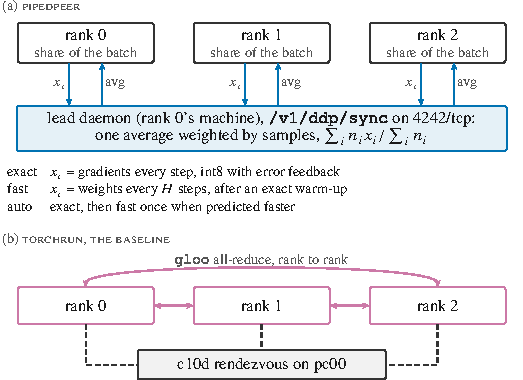
\includegraphics{../diagrams/tikz/pdf/ddp.pdf}
\par\vspace{2pt}{\color{black!55}\scriptsize\texttt{ddp}: single column, 3.49$\times$2.53\,in, System Design: Transparent Interception}
\caption{Data-parallel training. (a) Each PipedPeer rank posts to the lead daemon and receives one sample-weighted average; exact mode sends int8 gradients every step, fast mode weights every H steps. (b) The torchrun baseline meets at a c10d rendezvous and all-reduces between ranks over gloo.}
\label{fig:ddp}
\end{figure}

\begin{figure}[!htb]
\centering
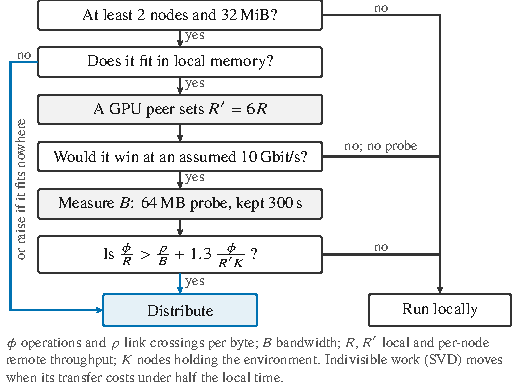
\includegraphics{../diagrams/tikz/pdf/cost.pdf}
\par\vspace{2pt}{\color{black!55}\scriptsize\texttt{cost}: single column, 3.49$\times$2.56\,in, System Design: The Cost Model}
\caption{The cost model as a cascade. Cheap tests run first; bandwidth is measured only when offloading could win at 10 Gbit/s. Work moves when Equation 2 holds or when it does not fit in local memory.}
\label{fig:cost}
\end{figure}

\begin{figure}[!htb]
\centering
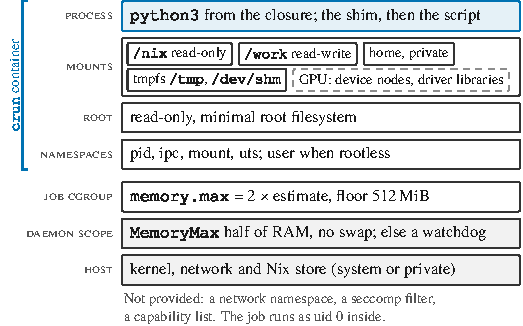
\includegraphics{../diagrams/tikz/pdf/sandbox.pdf}
\par\vspace{2pt}{\color{black!55}\scriptsize\texttt{sandbox}: single column, 3.49$\times$2.17\,in, System Design: Implementation}
\caption{The job sandbox. The closure is mounted read-only and the workspace read-write inside a crun container; a per-job cgroup and the daemon's own scope bound memory. The job shares the host network.}
\label{fig:sandbox}
\end{figure}

\begin{figure*}[!t]
\centering
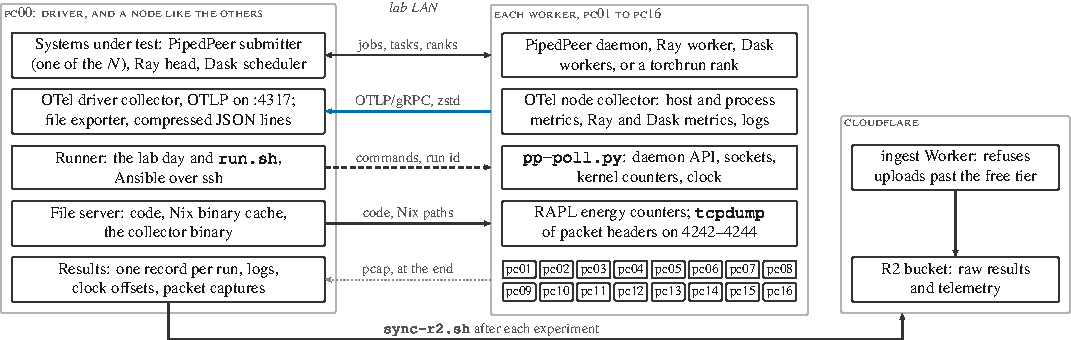
\includegraphics{../diagrams/tikz/pdf/lab.pdf}
\par\vspace{2pt}{\color{black!55}\scriptsize\texttt{lab}: double column, 7.14$\times$2.27\,in, Evaluation: Setup}
\caption{Lab campaign. pc00 runs the experiments over Ansible, hosts the Ray head, Dask scheduler and PipedPeer submitter, and collects OpenTelemetry from a collector on every PC into files; after each experiment the results go to R2 through an ingest Worker that refuses uploads past the free tier.}
\label{fig:lab}
\end{figure*}

\begin{figure}[!htb]
\centering
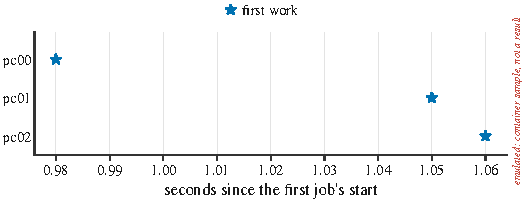
\includegraphics{figures-draft/eval-e14-staircase.pdf}
\par\vspace{2pt}{\color{black!55}\scriptsize\texttt{eval-e14-staircase}: single column, 3.49$\times$1.35\,in, Evaluation: Setup}
\caption{Curl to cluster (E14): for every PC, when it printed its LAB-PC line, answered SSH, had PipedPeer installed, joined, and first ran work of the day's first distributed job, relative to the head command on pc00. Dashed lines: cluster ready and first job.}
\label{fig:eval-e14-staircase}
\end{figure}

\begin{figure}[!htb]
\centering
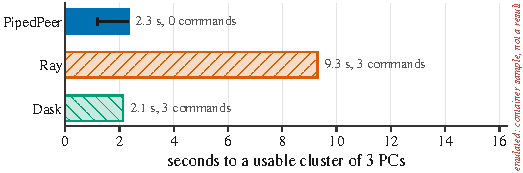
\includegraphics{figures-draft/eval-e17-ready.pdf}
\par\vspace{2pt}{\color{black!55}\scriptsize\texttt{eval-e17-ready}: single column, 3.49$\times$1.15\,in, Evaluation: Setup}
\caption{From nothing running to a cluster that accepts a job (E17): seconds from the first start command until the readiness check passed; the whisker reaches back to the last failed check. The number is the commands a user types after every boot.}
\label{fig:eval-e17-ready}
\end{figure}

\begin{figure}[!htb]
\centering
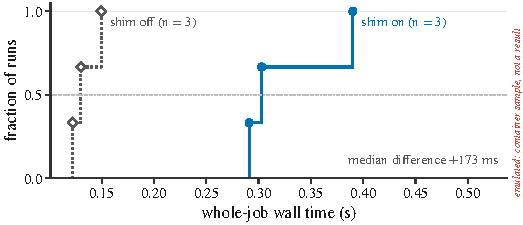
\includegraphics{figures-draft/eval-e7-overhead-cdf.pdf}
\par\vspace{2pt}{\color{black!55}\scriptsize\texttt{eval-e7-overhead-cdf}: single column, 3.49$\times$1.50\,in, Evaluation: Microbenchmarks (Q1, Q2)}
\caption{Cost of transparent interception (E7): CDF of the whole-job wall time of a script that does no parallel work, with the shim injected and without. The gap between the medians is the per-job overhead.}
\label{fig:eval-e7-overhead-cdf}
\end{figure}

\begin{figure}[!htb]
\centering
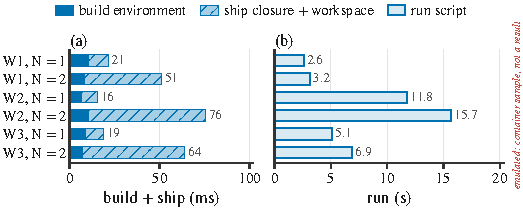
\includegraphics{figures-draft/eval-time-breakdown.pdf}
\par\vspace{2pt}{\color{black!55}\scriptsize\texttt{eval-time-breakdown}: single column, 3.49$\times$1.40\,in, Evaluation: Microbenchmarks (Q1, Q2)}
\caption{Where a PipedPeer job's time goes, from its own step records. (a) Building the Nix environment and shipping closure and workspace, in milliseconds; (b) running the script, in seconds. Median over repeats, warm environment cache.}
\label{fig:eval-time-breakdown}
\end{figure}

\begin{figure}[!htb]
\centering
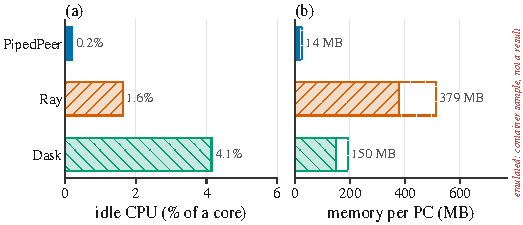
\includegraphics{figures-draft/eval-e17-footprint.pdf}
\par\vspace{2pt}{\color{black!55}\scriptsize\texttt{eval-e17-footprint}: single column, 3.49$\times$1.50\,in, Evaluation: Microbenchmarks (Q1, Q2)}
\caption{Idle cost of an installed cluster (E17), per PC, averaged over a quiet minute with no job: (a) CPU as a percentage of one core; (b) memory, proportional set size (bar) and resident set size (outline), of every process the system leaves running.}
\label{fig:eval-e17-footprint}
\end{figure}

\begin{figure}[!htb]
\centering
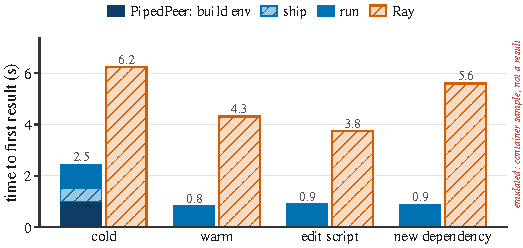
\includegraphics{figures-draft/eval-e19-ship.pdf}
\par\vspace{2pt}{\color{black!55}\scriptsize\texttt{eval-e19-ship}: single column, 3.49$\times$1.65\,in, Evaluation: Microbenchmarks (Q1, Q2)}
\caption{Time to first result while iterating on a script (E19), 16 PCs: the first run of a new environment (cold), the same again (warm), one constant edited, and one new dependency. PipedPeer's bar is split into environment build, ship, and the rest of the job. Median over repeats.}
\label{fig:eval-e19-ship}
\end{figure}

\begin{figure}[!htb]
\centering
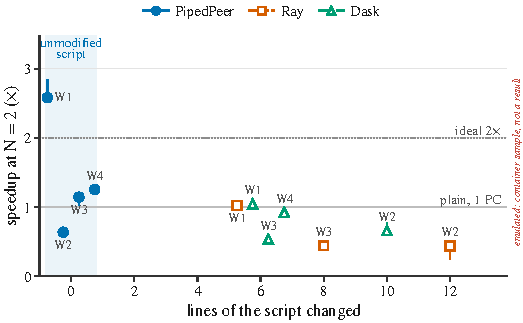
\includegraphics{figures-draft/eval-frontier.pdf}
\par\vspace{2pt}{\color{black!55}\scriptsize\texttt{eval-frontier}: single column, 3.49$\times$2.15\,in, Evaluation: End-to-end runs (Q3)}
\caption{Porting cost against payoff. Each point is one workload on one system at the largest N; the vertical bar is the interquartile range over repeats. PipedPeer runs the unmodified script (zero lines changed); Ray and Dask need a port.}
\label{fig:eval-frontier}
\end{figure}

\begin{figure*}[!t]
\centering
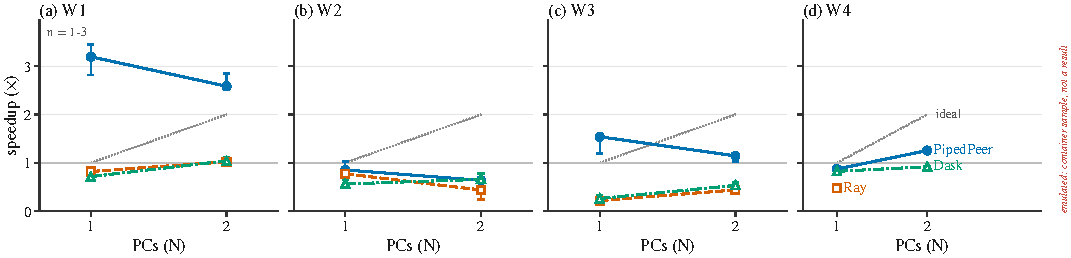
\includegraphics{figures-draft/eval-strong-scaling.pdf}
\par\vspace{2pt}{\color{black!55}\scriptsize\texttt{eval-strong-scaling}: double column, 7.14$\times$1.72\,in, Evaluation: End-to-end runs (Q3)}
\caption{Strong scaling. Speedup over plain Python on one PC (median; bars are the IQR over repeats) against the number of PCs N. The dotted line is ideal linear speedup; the grey line is parity with plain Python. Panels share the y axis.}
\label{fig:eval-strong-scaling}
\end{figure*}

\begin{figure}[!htb]
\centering
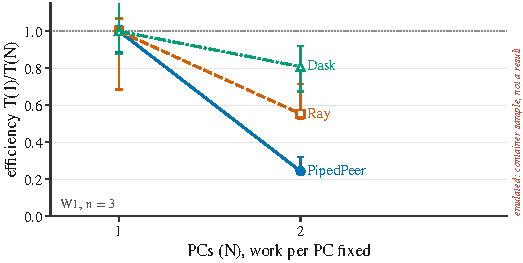
\includegraphics{figures-draft/eval-weak-scaling.pdf}
\par\vspace{2pt}{\color{black!55}\scriptsize\texttt{eval-weak-scaling}: single column, 3.49$\times$1.75\,in, Evaluation: End-to-end runs (Q3)}
\caption{Weak scaling of W1: the work grows with N, so a perfect system holds efficiency T(1)/T(N) at 1.0 (dotted). Median and IQR over repeats.}
\label{fig:eval-weak-scaling}
\end{figure}

\begin{figure*}[!t]
\centering
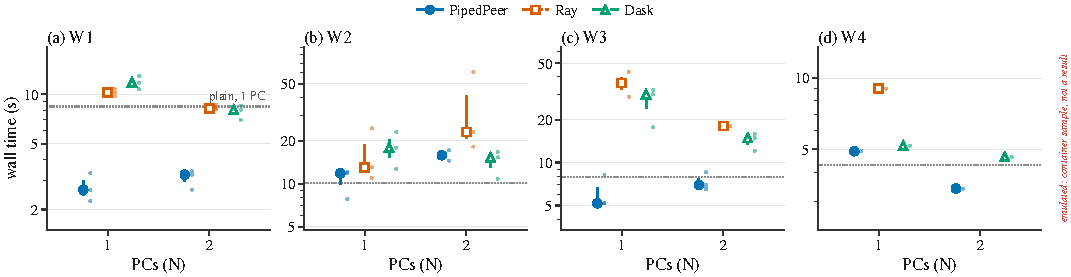
\includegraphics{figures-draft/eval-wall-time.pdf}
\par\vspace{2pt}{\color{black!55}\scriptsize\texttt{eval-wall-time}: double column, 7.14$\times$1.85\,in, Evaluation: End-to-end runs (Q3)}
\caption{Wall time per workload, system and N. The marker is the median, the bar the IQR, and the small dots are the individual repeats; the dotted line is plain Python on one PC. Lower is better; log y axis, each panel with its own range.}
\label{fig:eval-wall-time}
\end{figure*}

\begin{figure}[!htb]
\centering
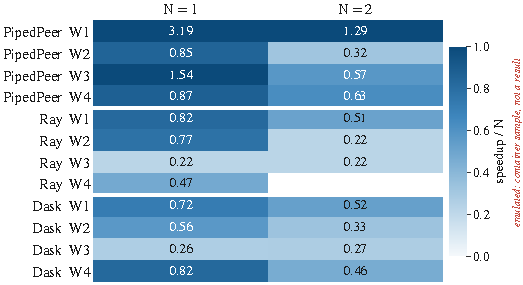
\includegraphics{figures-draft/eval-efficiency-heatmap.pdf}
\par\vspace{2pt}{\color{black!55}\scriptsize\texttt{eval-efficiency-heatmap}: single column, 3.49$\times$1.90\,in, Evaluation: End-to-end runs (Q3)}
\caption{Parallel efficiency (speedup over plain Python divided by N) for every system, workload and N. 1.00 is linear scaling. Darker is better; values are printed so the figure reads in greyscale.}
\label{fig:eval-efficiency-heatmap}
\end{figure}

\begin{figure}[!htb]
\centering
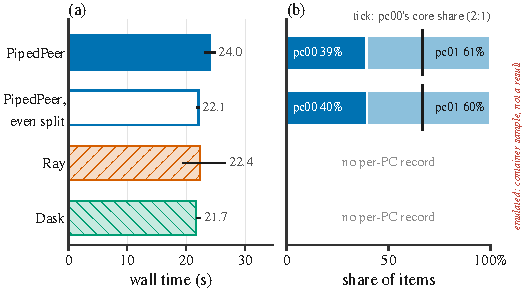
\includegraphics{figures-draft/eval-e4-heterogeneous.pdf}
\par\vspace{2pt}{\color{black!55}\scriptsize\texttt{eval-e4-heterogeneous}: single column, 3.49$\times$1.95\,in, Evaluation: End-to-end runs (Q3)}
\caption{Unequal PCs (E4). (a) Wall time, median and IQR. (b) Share of the items each PC computed in one representative run; the black tick is the first PC's share of the cores. The even split is PipedPeer with placement by head count instead of measured speed.}
\label{fig:eval-e4-heterogeneous}
\end{figure}

\begin{figure}[!htb]
\centering
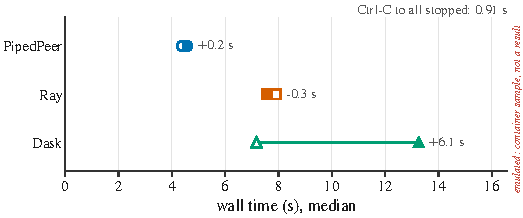
\includegraphics{figures-draft/eval-e6-kill.pdf}
\par\vspace{2pt}{\color{black!55}\scriptsize\texttt{eval-e6-kill}: single column, 3.49$\times$1.45\,in, Evaluation: End-to-end runs (Q3)}
\caption{One worker killed with kill -9 mid-run (E6). Hollow: no fault; filled: killed. The label is the added wall time; every run returned the correct result unless marked.}
\label{fig:eval-e6-kill}
\end{figure}

\begin{figure*}[!t]
\centering
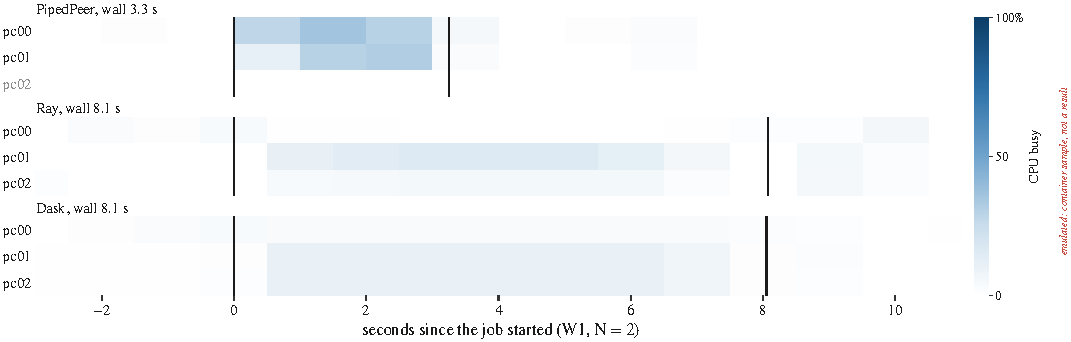
\includegraphics{figures-draft/eval-cpu-heatmap.pdf}
\par\vspace{2pt}{\color{black!55}\scriptsize\texttt{eval-cpu-heatmap}: double column, 7.14$\times$2.28\,in, Evaluation: End-to-end runs (Q3)}
\caption{CPU utilisation of every PC during one W1 run at the largest N (OTel host or cgroup CPU time; busy cores over logical cores, 0.5 s bins). The vertical lines mark the job's start and end; PCs the run did not use are labelled in grey.}
\label{fig:eval-cpu-heatmap}
\end{figure*}

\begin{figure*}[!t]
\centering
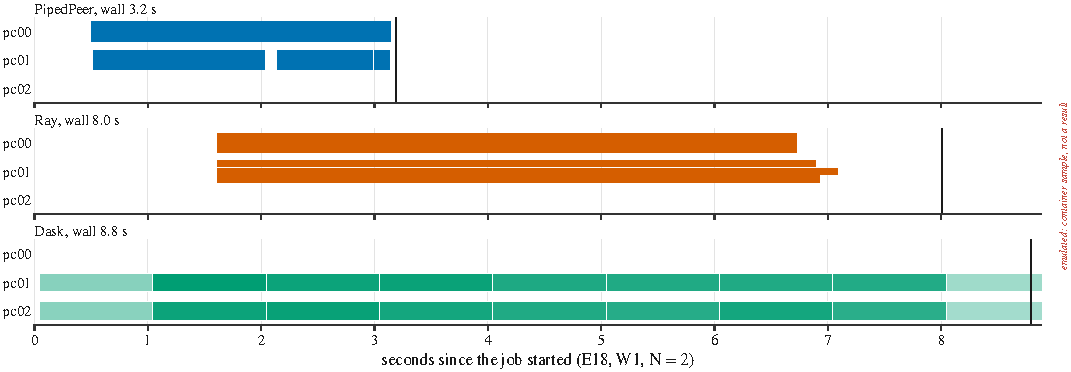
\includegraphics{figures-draft/eval-swimlanes.pdf}
\par\vspace{2pt}{\color{black!55}\scriptsize\texttt{eval-swimlanes}: double column, 7.14$\times$2.48\,in, Evaluation: End-to-end runs (Q3)}
\caption{Where the work ran. Each bar is one chunk of items on the PC that computed it, from each system's own records (PipedPeer's receipt, Ray's timeline, Dask's scheduler). Dask records tasks per second, drawn as one-second cells shaded by count. Rows within a PC are concurrent chunks.}
\label{fig:eval-swimlanes}
\end{figure*}

\begin{figure}[!htb]
\centering
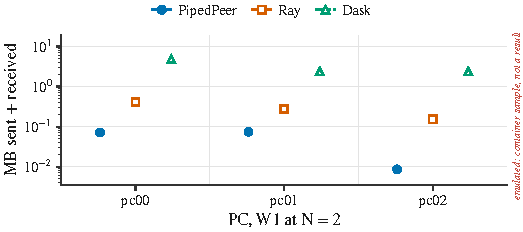
\includegraphics{figures-draft/eval-net-bytes.pdf}
\par\vspace{2pt}{\color{black!55}\scriptsize\texttt{eval-net-bytes}: single column, 3.49$\times$1.55\,in, Evaluation: End-to-end runs (Q3)}
\caption{Network traffic per PC: bytes sent plus received on the lab interface during one W1 run per system at the largest N (OTel system.network.io). Log y axis; pc00 submits the job and hosts the Ray head and the Dask scheduler.}
\label{fig:eval-net-bytes}
\end{figure}

\begin{figure}[!htb]
\centering
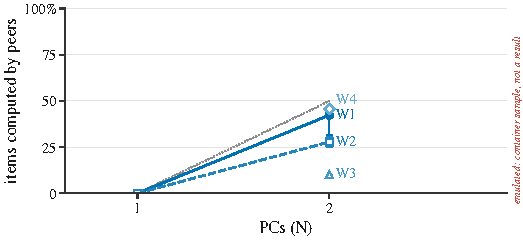
\includegraphics{figures-draft/eval-offload-share.pdf}
\par\vspace{2pt}{\color{black!55}\scriptsize\texttt{eval-offload-share}: single column, 3.49$\times$1.60\,in, Evaluation: End-to-end runs (Q3)}
\caption{How much work PipedPeer moved off the submitting PC: the share of mapped items computed by peers (from the shim's receipt), median and range over repeats. The dotted line is an even share (N-1)/N.}
\label{fig:eval-offload-share}
\end{figure}

\begin{figure*}[!t]
\centering
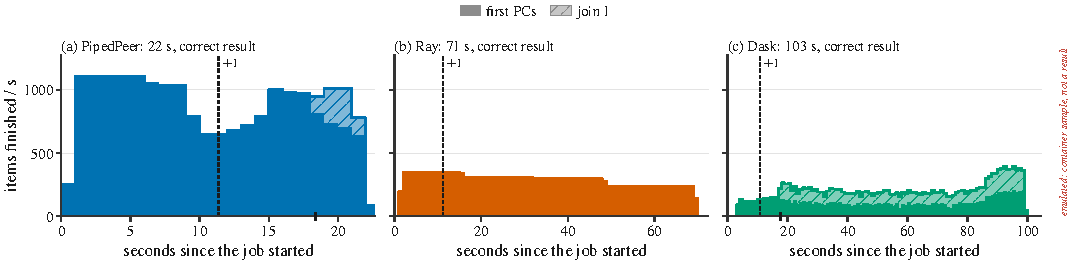
\includegraphics{figures-draft/eval-e12-join.pdf}
\par\vspace{2pt}{\color{black!55}\scriptsize\texttt{eval-e12-join}: double column, 7.14$\times$1.75\,in, Evaluation: End-to-end runs (Q3)}
\caption{Elastic join (E12). Items finished per second, stacked by cohort: the PCs the job started on, then each group that joined (dashed line, labelled with the PCs added). A cohort that stays at zero is a system that never used the PCs that joined. Panels share the y axis.}
\label{fig:eval-e12-join}
\end{figure*}

\begin{figure*}[!t]
\centering
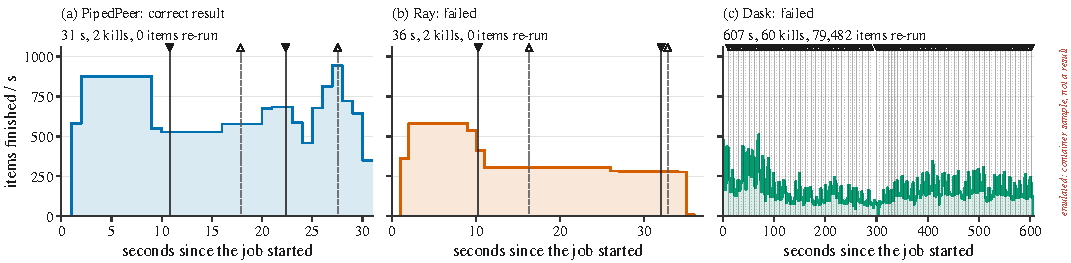
\includegraphics{figures-draft/eval-e13-churn.pdf}
\par\vspace{2pt}{\color{black!55}\scriptsize\texttt{eval-e13-churn}: double column, 7.14$\times$1.75\,in, Evaluation: End-to-end runs (Q3)}
\caption{Churn (E13): a worker is killed with kill -9 periodically (solid line, filled triangle) and restarted a few seconds later (dotted line, hollow triangle). Items finished per second over all PCs; each panel gives the outcome, the wall time against the same job without churn, and the items computed twice.}
\label{fig:eval-e13-churn}
\end{figure*}

\begin{figure}[!htb]
\centering
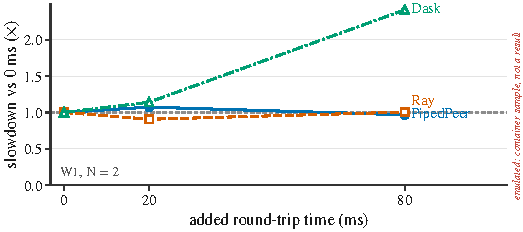
\includegraphics{figures-draft/eval-e15-network.pdf}
\par\vspace{2pt}{\color{black!55}\scriptsize\texttt{eval-e15-network}: single column, 3.49$\times$1.55\,in, Evaluation: End-to-end runs (Q3)}
\caption{Network sensitivity (E15): W1 wall time with netem delay added between every pair of PCs, relative to the same system with no added delay. Median; bars span the IQR over repeats.}
\label{fig:eval-e15-network}
\end{figure}

\begin{figure*}[!t]
\centering
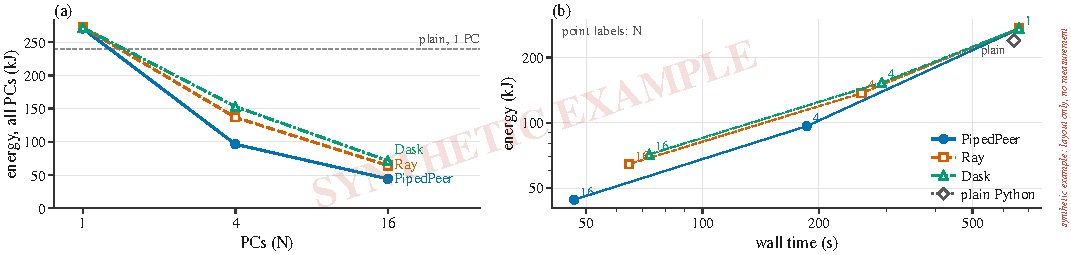
\includegraphics{figures-draft/eval-e16-energy.pdf}
\par\vspace{2pt}{\color{black!55}\scriptsize\texttt{eval-e16-energy}: double column, 7.14$\times$1.70\,in, Evaluation: End-to-end runs (Q3)}
\caption{Energy to solution (E16), W1, package energy from RAPL summed over all 17 PCs, idle ones included. (a) Energy against N; the dashed line is plain Python on one PC. (b) Energy against wall time, both log: lower left is faster and cheaper.}
\label{fig:eval-e16-energy}
\end{figure*}

\begin{figure*}[!t]
\centering
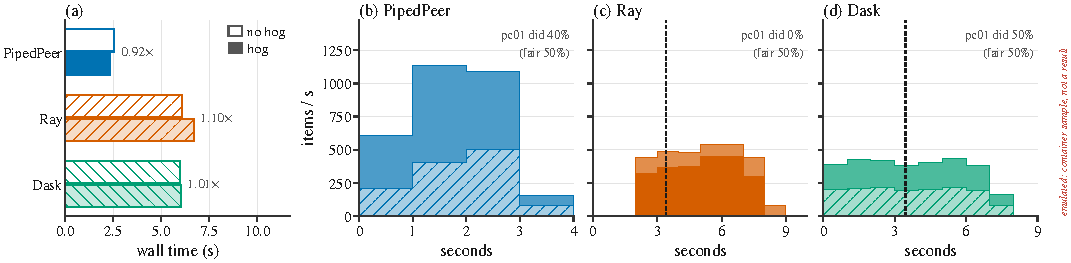
\includegraphics{figures-draft/eval-e18-straggler.pdf}
\par\vspace{2pt}{\color{black!55}\scriptsize\texttt{eval-e18-straggler}: double column, 7.14$\times$1.75\,in, Evaluation: End-to-end runs (Q3)}
\caption{Noisy neighbour (E18): busy loops on half the cores of one PC, started a few seconds into W1. (a) Wall time without (hollow) and with (filled) the hog; the label is the slowdown. (b-d) Items finished per second in the hog run, stacked per PC, the hogged PC hatched; the dashed line is the hog's start. Panels (b-d) share the y axis.}
\label{fig:eval-e18-straggler}
\end{figure*}

\begin{figure}[!htb]
\centering
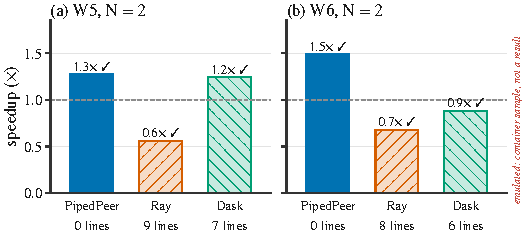
\includegraphics{figures-draft/eval-e20-unmodified.pdf}
\par\vspace{2pt}{\color{black!55}\scriptsize\texttt{eval-e20-unmodified}: single column, 3.49$\times$1.60\,in, Evaluation: End-to-end runs (Q3)}
\caption{Unmodified pandas and scikit-learn (E20). W5 fits a model per pandas group through joblib; W6 is cross\_val\_score with n\_jobs=-1. Speedup over plain Python on one PC; the tick above each bar marks that every run matched plain Python, and the line under each name is the number of script lines changed.}
\label{fig:eval-e20-unmodified}
\end{figure}

\begin{figure*}[!t]
\centering
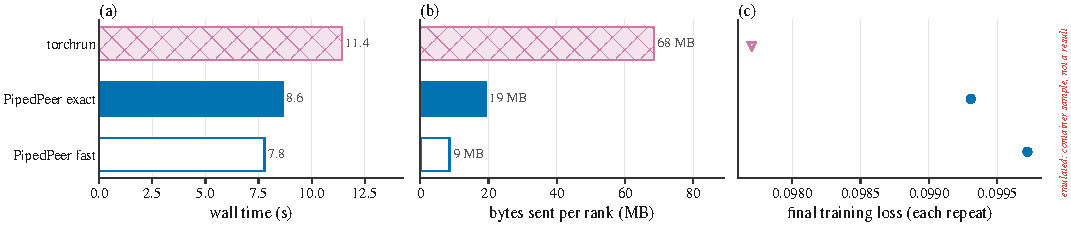
\includegraphics{figures-draft/eval-e8-training.pdf}
\par\vspace{2pt}{\color{black!55}\scriptsize\texttt{eval-e8-training}: double column, 7.14$\times$1.50\,in, Evaluation: Training (Q4)}
\caption{Data-parallel training (E8). (a) Wall time, median and IQR. (b) Bytes each rank sent. (c) Final training loss of each repeat. Exact averages gradients every step; fast averages weights every few steps.}
\label{fig:eval-e8-training}
\end{figure*}

